\vspace{-0.2cm}
\subsection{Experimental Evaluation}
\label{sec:scaling_exps}
\vspace{-0.2cm}

\begin{figure}[t]
    \centering
    \begin{minipage}{0.65\linewidth}
 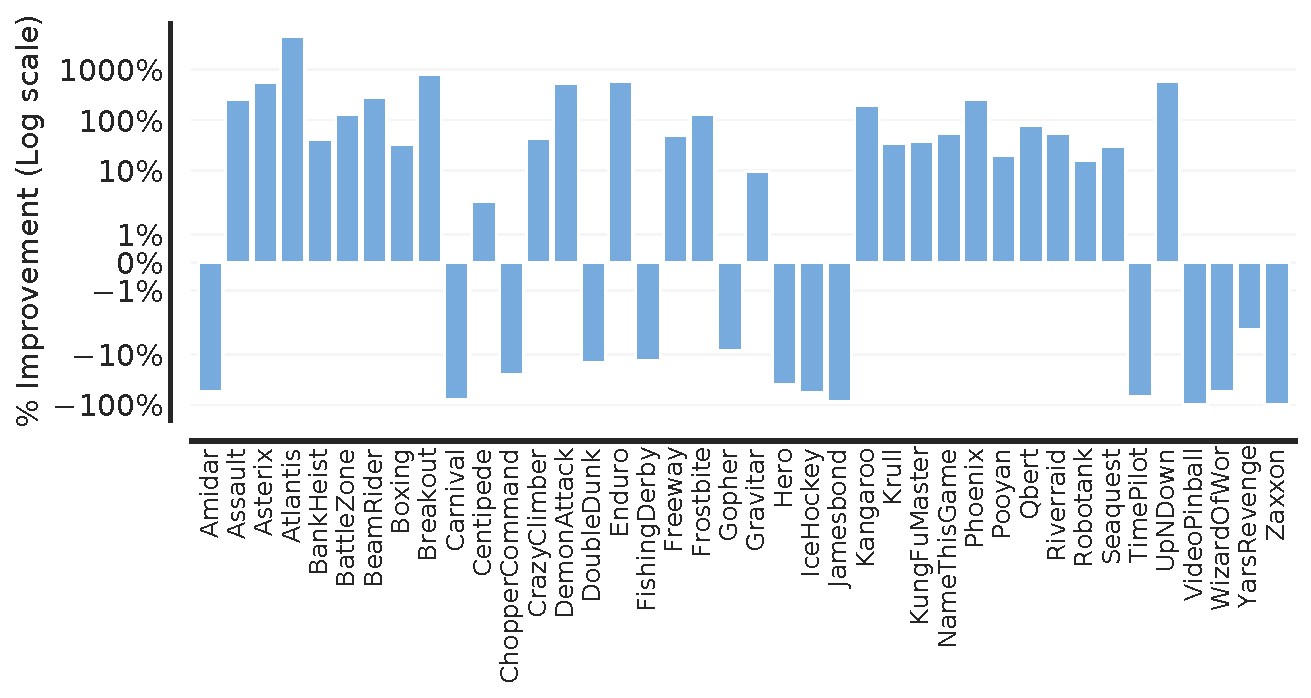
\includegraphics[width=\linewidth]{chapters/scaled_ql/figures/percent_improvement_over_DT.pdf}
    \end{minipage}
    \hfill
    \begin{minipage}{0.34\linewidth}
    \vspace{-0.2cm}
 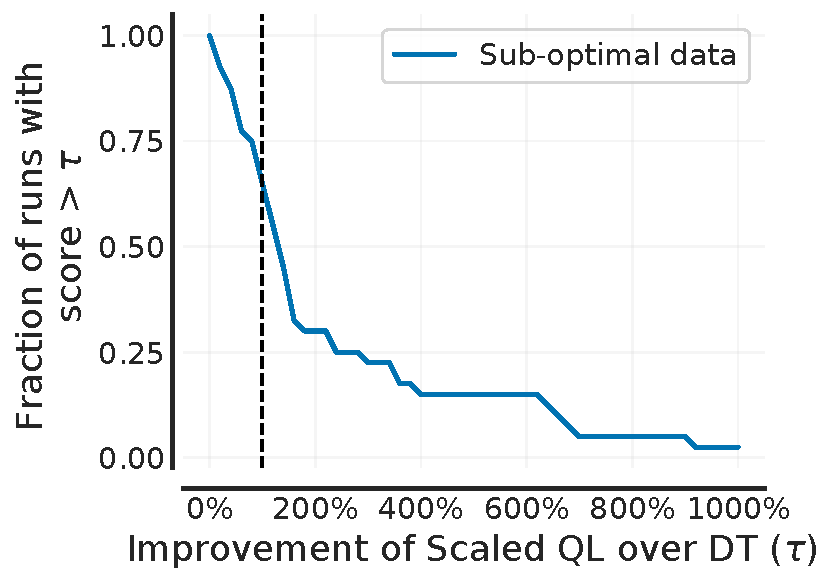
\includegraphics[width=\linewidth]{chapters/scaled_ql/figures/pp_profile_ql_dt.pdf}
    \end{minipage}
    \vspace{-0.4cm}
    \caption{\textbf{Comparing Scaled QL to DT} on all training games on the sub-optimal dataset.}
    \label{fig:percent_improvement}
    \vspace{-0.5cm}
\end{figure}

In our experiments, we study how our approach, scaled Q-learning, can simultaneously learn from sub-optimal and optimal data collected from 40 different Atari games. 
We compare the resulting multi-task policies to behavior cloning~(BC) with same architecture as scaled QL, and the prior state-of-the-art method based on decision transformers (DT)~\citep{chen2021decision}, which utilize return-conditioned supervised learning with large transformers~\citep{lee2022multi}, and have been previously proposed for addressing this task. 
We also study the efficacy of the multi-task initialization produced by scaled Q-learning in facilitating rapid transfer to new games via both offline and online fine-tuning, in comparison to state-of-the-art self-supervised representation learning methods and other prior approaches. Our goal is to answer the following questions: \textbf{(1)} How do our proposed design decisions impact performance scaling with high-capacity models?, \textbf{(2)} Can scaled QL more effectively leverage higher model capacity compared to na\"ive instantiations of Q-learning?, \textbf{(3)} Do the representations learned by scaled QL transfer to new games? We will answer these questions in detail through multiple experiments in the coming sections, but we will first summarize our main results below.


\textbf{Main empirical findings.} Our main results are summarized in Figures~\ref{fig:suboptimal_offline} and \ref{fig:main_results}. These figures show the performance of scaled QL, multi-game decision transformers~\citep{lee2022multi} (marked as ``DT''), a prior method based on supervised learning via return conditioning, and standard behavioral cloning baselines (marked as ``BC'') in the two settings discussed previously, where we must learn from: (i) near optimal data, and (ii) sub-optimal data obtained from the initial 20\% segment of the replay buffer (see our discussion about the problem setup). See Figure~\ref{fig:percent_improvement} for a direct comparison between DT and BC.


\begin{wrapfigure}{r}{0.5\linewidth}
    \vspace{-0.5cm}
    \centering
    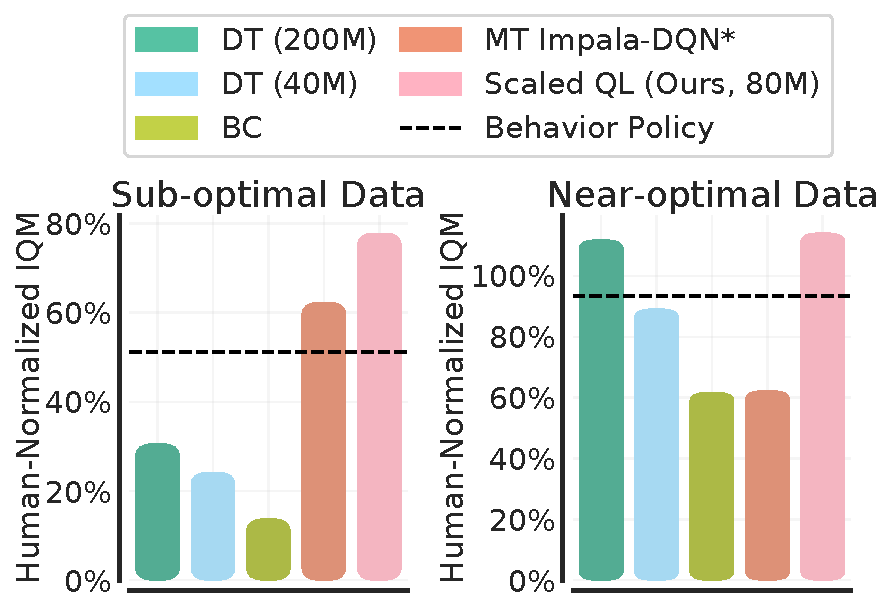
\includegraphics[width=0.95\linewidth]{chapters/scaled_ql/combnined_data_results_iqm.pdf}
    \vspace{-0.25cm}
    \caption{\footnotesize{\textbf{Offline scaled conservative Q-learning vs other prior methods} with near-optimal data and sub-optimal data. Scaled QL outperforms the best DT model, attaining an IQM human-normalized score of \textbf{114.1\%} on the near-optimal data and \textbf{77.8\%} on the sub-optimal data, compared to 111.8\% and 30.6\% for DT, respectively.}}
    \label{fig:main_results}
    \vspace{-0.5cm}
\end{wrapfigure}

In the more challenging sub-optimal data setting, scaled QL attains a performance of \textbf{77.8\%} IQM human-normalized score, although trajectories in the sub-optimal training dataset only attain 51\% IQM human-normalized score. Scaled QL also outperforms the prior DT approach by \textbf{2.5 times} on this dataset, even though the DT model has more than twice as many parameters and uses data augmentation, compared to scaled QL. 

In the $2^{nd}$ setting with near-optimal data, where the training dataset already contains expert trajectories, scaled QL with 80M parameters still outperforms the DT approach with 200M parameters, although the gap in performance is small (3\% in IQM performance, and 20\% on median performance). 
Overall, these results show that scaled QL is an effective approach for learning from large multi-task datasets, for a variety of data compositions including sub-optimal datasets, where we must stitch useful segments of suboptimal trajectories to perform well, and near-optimal datasets, where we should attempt to mimic the best behavior in the offline dataset. 

To the best of our knowledge, these results represent the largest performance improvement over the average performance in the offline dataset on such a challenging problem. We will now present experiments that show that offline Q-learning scales and generalizes.

\begin{figure}[h]
\centering
\vspace{-0.2cm}
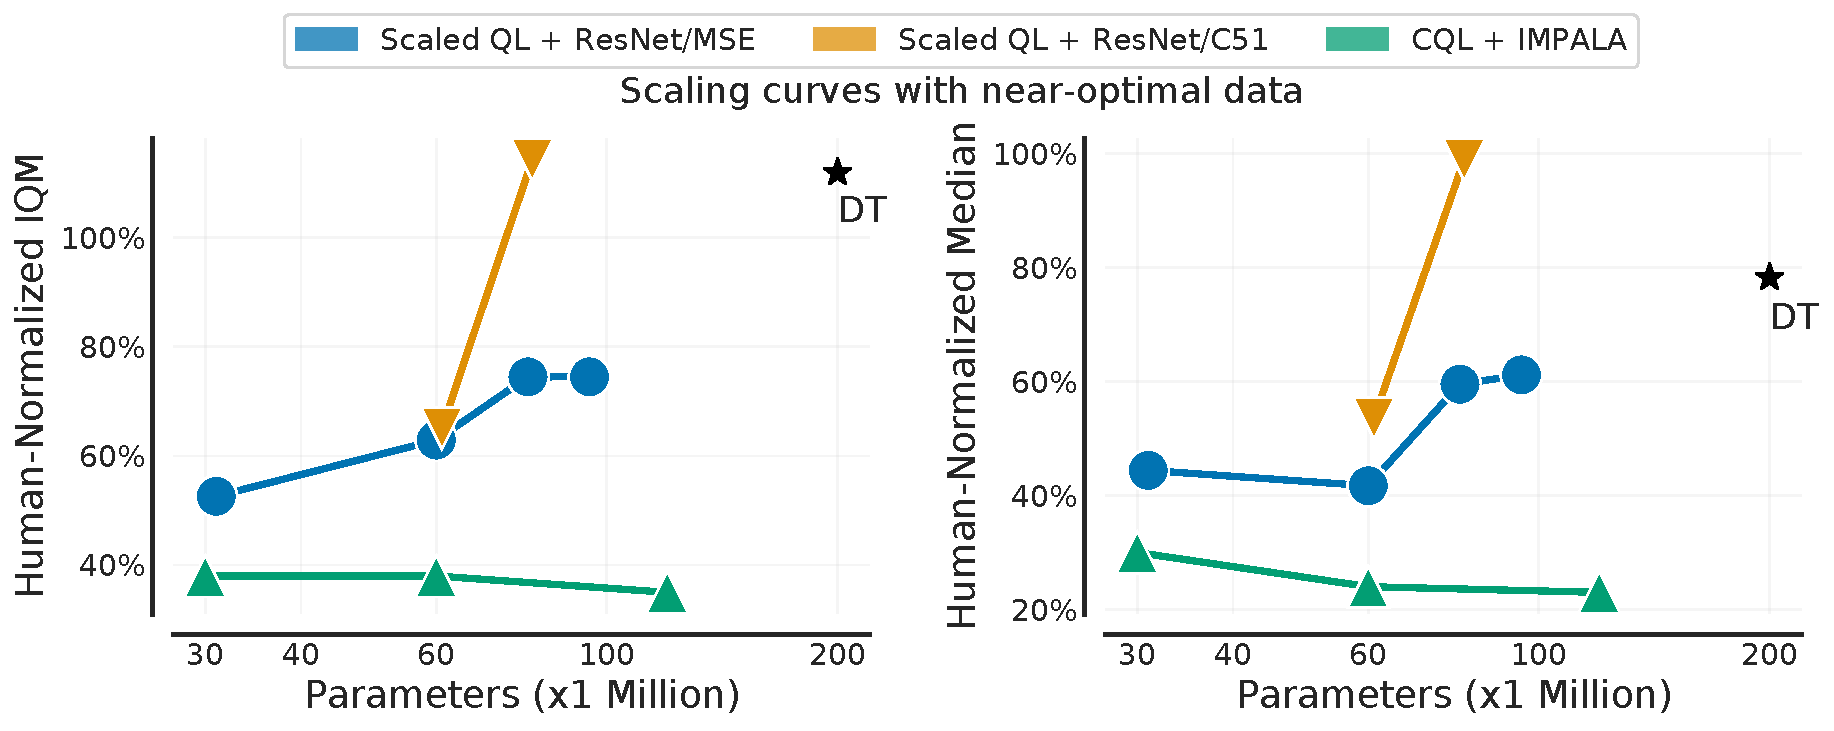
\includegraphics[width=0.75\linewidth]{chapters/scaled_ql/figures/scaling_plot_params_with_dt.pdf}
\vspace{-0.2cm}
\caption{\footnotesize{\textbf{Scaling trends for offline Q-learning.} Observe that while the performance of scaled QL instantiated with IMPALA architectures~\citep{espeholt2018impala} degrades as we increase model size, the performance of scaled QL utilizing the ResNets described in Section~\ref{sec:scaledql_method} continues to increase as model capacity increases. This is true for both an MSE-style TD error as well as for the categorical TD error used by C51 (which performs better on an absolute scale). The CQL + IMPALA performance numbers are from~\citep{lee2022multi}.}
}
\label{fig:scaling}
\vspace{-0.2cm}
\end{figure}

\vspace{-0.2cm}
\subsubsection{Does Offline Conservative Q-Learning Scale Favorably?}
\vspace{-0.2cm}
One of the primary goals of this chapter was to understand if scaled Q-learning is able to leverage the benefit of higher capacity architectures. Recently, \citet{lee2022multi} found that the performance of CQL with the IMPALA architecture does not improve with larger model sizes and may even degrade with larger model sizes. To verify if scaled Q-learning can address this limitation, we compare our value-based offline RL approach with a variety of model families: \textbf{(a)} IMPALA family~\citep{espeholt2018impala}: three IMPALA models with varying widths ($4, 8, 16$) whose performance numbers are taken directly from \citet{lee2022multi} (and was consistent with our preliminary experiments), 
%%AK: check if this is the standard naming or not?
\textbf{(b)} ResNet 34, 50, 101 and 152 from the ResNet family, modified to include group normalization and learned spatial embeddings.%, and \textbf{(c)} ViT-Base and ViT-Large from the vision transformer family, similar to decision transformers. 
These architectures include both small and large networks, spanning a wide range from 1M to 100M parameters. As a point of reference, we use the scaling trends of the multi-game decision transformer and BC approaches from \citet{lee2022multi}.
%%SL.9.27: if we don't end up including vit, make sure to revise the above discussion

Observe in Figure~\ref{fig:scaling} that the performance of scaled Q-learning improves as the underlying Q-function model size grows. Even though the standard mean-squared error formulation of TD error results in worse absolute performance than C51 (blue vs orange), for both of these versions, the performance of scaled Q-learning increases as the models become larger. This result indicates that value-based offline RL methods can scale favorably, and give rise to better results, but this requires carefully picking a model family. This also explains the findings from \citet{lee2022multi}: while this prior work observed that CQL with IMPALA scaled poorly as model size increases, they also observed that the performance of return-conditioned RL instantiated with IMPALA architectures also degraded with higher model sizes. Combined with the results in Figure~\ref{fig:scaling} above, this suggests that poor scaling properties of offline RL can largely be attributed to the choice of IMPALA architectures, which may not work well in general even for supervised learning methods (like return-conditioned BC).


\vspace{-0.2cm}
\subsubsection{Can Offline RL Learn Useful Initializations that Enable Fine-Tuning?}
\label{sec:ft_off_on}
\vspace{-0.2cm}

Next, we study how multi-task training on multiple games via scaled QL can learn general-purpose representations that can enable \emph{rapid} fine-tuning to new games. We study this question in two scenarios: fine-tuning to a new game via offline RL with a small amount of held-out data (1\% uniformly subsampled datasets from DQN-Replay~\citep{agarwal2019optimistic}), and finetuning to a new game mode via sample-efficient online RL initialized from our multi-game offline Q-function. For finetuning, we transfer the weights from the visual encoder and reinitialize the downstream feed-forward component (Figure~\ref{fig:overview}). For both of these scenarios, we utilize a ResNet101 Q-function trained via the methodology in Section~\ref{sec:scaledql_method}, using C51 and feature normalization.

\begin{figure}[t]
    \centering
    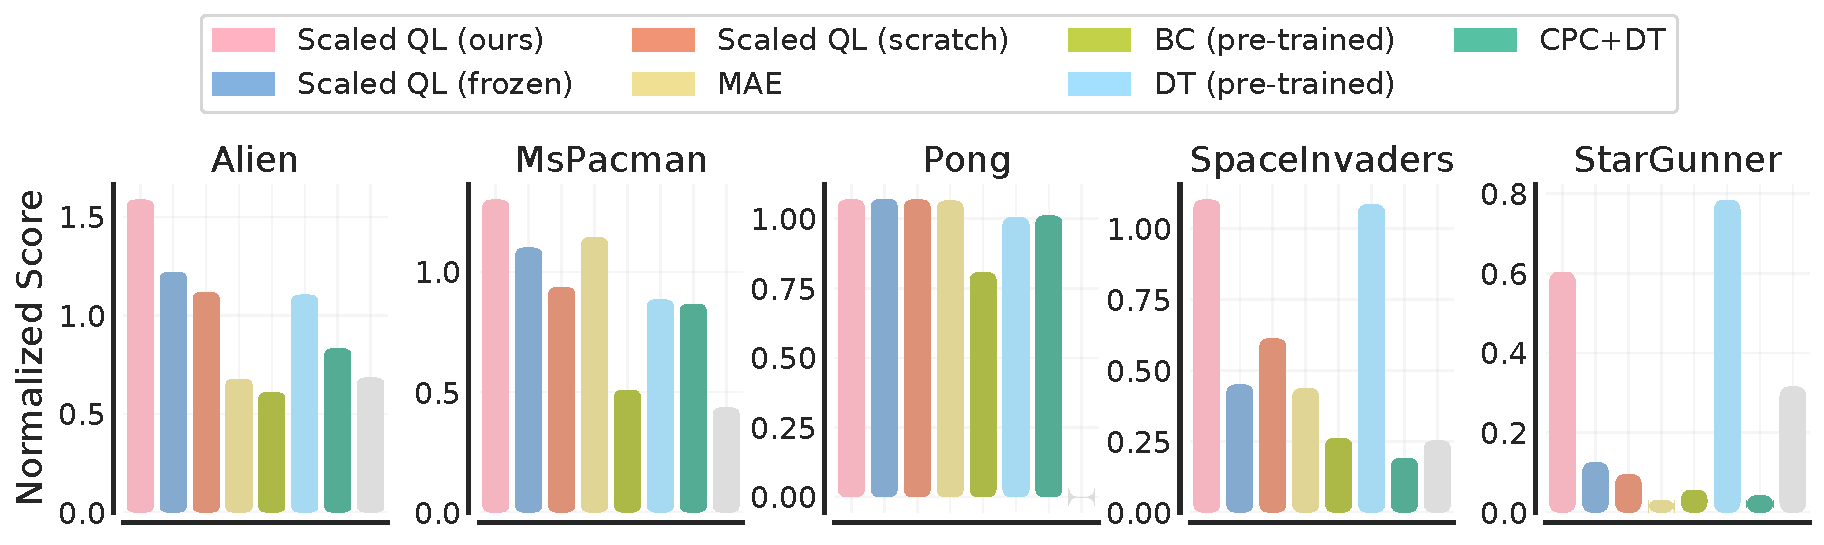
\includegraphics[width=0.99\linewidth]{chapters/scaled_ql/figures/offline_ft.pdf}
    \vspace{-0.25cm}
    \caption{\footnotesize{\textbf{Offline fine-tuning} performance on unseen games trained with 1\% of held-out game's data, measured in terms of DQN-normalized score, following \citep{lee2022multi}. On average, pre-training with scaled QL outperforms other methods by \textbf{82\%}. Furthermore, scaled QL improves over scaled QL (scratch) by 45\%, indicating that the representations learned by scaled QL during multi-game pre-training are useful for transfer. Self-supervised representation learning (CPC, MAE) alone does not attain good fine-tuning performance.}}
    \label{fig:offline_ft}
    \vspace{-0.3cm}
\end{figure}
%%AK: not having baselines para here, since the comparisons are different

\textbf{Scenario 1 (Offline fine-tuning)}: First, we present the results for fine-tuning in an offline setting: following the protocol from \citet{lee2022multi}, we use the pre-trained representations to rapidly learn a policy for a novel game using limited offline data (1\% of the experience of an online DQN run). In Figure~\ref{fig:offline_ft}, we present our results for offline fine-tuning on 5 games from \citet{lee2022multi}, \textsc{Alien, MsPacman, Space Invaders, StarGunner} and \textsc{Pong}, alongside the prior approach based on decision transformers (``DT (pre-trained)''), and fine-tuning using pre-trained representations learned from state-of-the-art self-supervised representation learning methods such as contrastive predictive coding (CPC)~\citep{oord2018representation} and masked autoencoders (MAE)~\citep{he2111masked}. For CPC performance, we use the baseline reported in \citet{lee2022multi}. MAE is a more recent self-supervised approach that we find generally outperformed CPC in this comparison. For MAE, we first pretrained a vision transformer~(ViT-Base)~\citep{dosovitskiy2020image} encoder with 80M parameters trained via a reconstruction loss on observations from multi-game Atari dataset and freeze the encoder weights as done in prior work~\citep{xiao2022masked}. 
Then, with this frozen visual encoder, we used the same feed forward architecture, Q-function parameterization, and training objective (CQL with C51) as scaled QL to finetune the MAE network. We also compare to baseline methods that do not utilize any multi-game pre-training (DT (scratch) and Scaled QL (scratch)). 

\textbf{Results.} Observe in Figure~\ref{fig:offline_ft} that multi-game pre-training via scaled QL leads to the best fine-tuning performance and improves over prior methods, including decision transformers trained from scratch. %, by XX\% in aggregate. 
Importantly, we observe \emph{positive transfer} to new games via scaled QL. Prior works~\citep{badia2020agent57}
running multi-game Atari (primarily in the online setting) have generally observed negative transfer across Atari games. We show for the first time that pre-trained representations from Q-learning enable positive transfer to novel games that significantly outperforms return-conditioned supervised learning methods and dedicated representation learning approaches.

\textbf{Scenario 2 (Online fine-tuning)}: Next, we study the efficacy of the learned representations in enabling online fine-tuning. While deep RL agents on ALE are typically trained on default game modes~(referred to as $m0d0$), we utilize new \emph{variants} of the ALE games designed to be challenging for humans~\citep{machado18sticky} for online-finetuning. We investigate whether multi-task training on the 40 default game variants can enable fast online adaptation to these never-before-seen variants. In contrast to offline fine-tuning (Scenario 1), this setting tests whether scaled QL can also provide a good initialization for online data collection and learning, for closely related but different tasks. Following \citet{farebrother2018generalization}, we use the same \emph{variants} investigated in this prior work: $\textsc{Breakout}$, $\textsc{Hero}$, and $\textsc{Freeway}$, which we visualize in Figure~\ref{fig:online_ft}~(left).
To disentangle the performance gains from multi-game pre-training and the choice of Q-function architecture, we compare to a baseline approach (``scaled QL (scratch)'') that utilizes an identical Q-function architecture as pre-trained scaled QL, but starts from a random initialization. As before, we also evaluate fine-tuning performance using the representations obtained via masked auto-encoder pre-training~\citep{he2111masked,xiao2022masked}. We also compare to a single-game DQN performance attained after training for 50M steps, $16\times$ more transitions than what is allowed for scaled QL, as reported by \citet{farebrother2018generalization}.

\textbf{Results}. Observe in Figure~\ref{fig:online_ft} that fine-tuning from the multi-task initialization learned by scaled QL significantly outperforms training from scratch as well as the single-game DQN run trained with \textbf{16x} more data. Fine-tuning with the frozen representations learned by MAE performs poorly, which we hypothesize is due to differences in game dynamics and subtle changes in observations, which must be accurately accounted for in order to learn optimal behavior~\citep{dean2022don}. Our results confirm that offline Q-learning can both effectively benefit from higher-capacity models and learn multi-task initializations that enable sample-efficient transfer to new games. 


\begin{figure}[t]
    \centering
        
\includegraphics[width=0.9\linewidth]{chapters/scaled_ql/figures/legend_online_ft.pdf}
        \vspace{-0.1cm}
        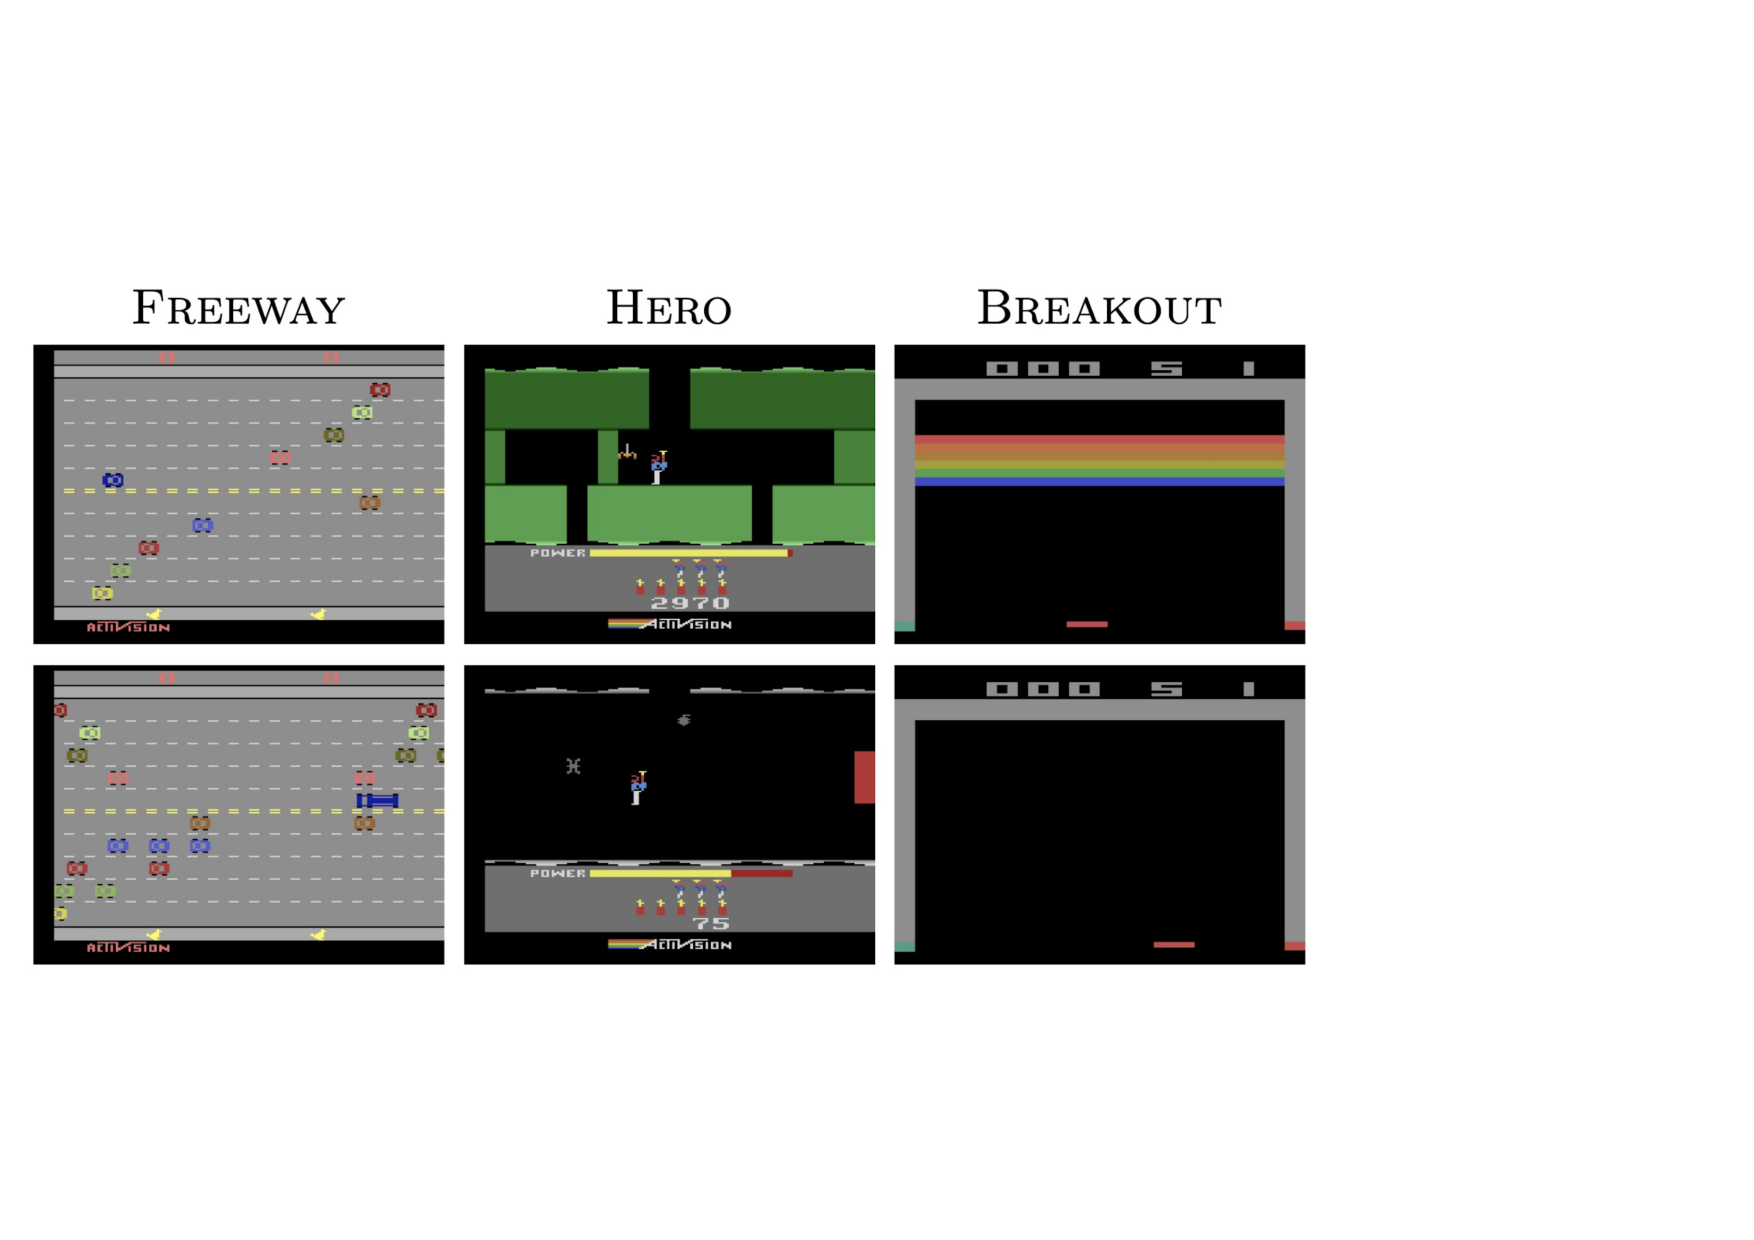
\includegraphics[width=0.35\linewidth]{chapters/scaled_ql/figures/atari_modes_3games.pdf}
        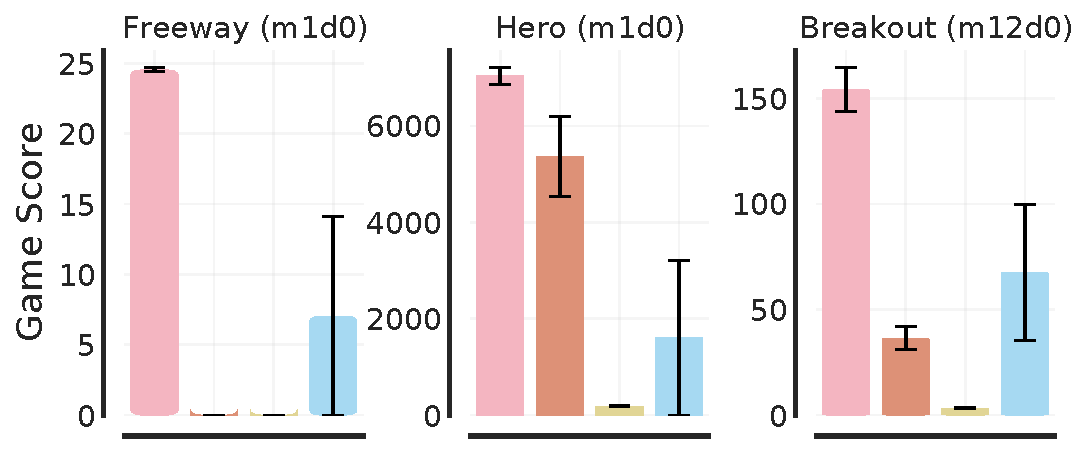
\includegraphics[width=0.5\linewidth]{chapters/scaled_ql/figures/online_ft_3_games.pdf}
    \vspace{-0.1cm}
    \caption{\footnotesize{\textbf{Online fine-tuning} results on unseen game \emph{variants}. \textbf{Left}. The top row shows default variants and the bottom row shows unseen variants evaluated for transfer: Freeway’s mode 1 adds buses, more vehicles, and increases velocity; Hero’s mode 1 starts the agent at level 5; Breakout’s mode 12 hides all bricks unless the ball has recently collided with a brick. \textbf{Right}. We fine-tune all methods except single-game DQN for 3M online frames (as we wish to test fast online adaptation). Error bars show minimum and maximum scores across 2 runs while the bar shows their average. Observe that scaled QL significantly outperforms learning from scratch and single-game DQN with 50M online frames. Furthermore, scaled QL also outperforms RL fine-tuning on representations learned using masked auto-encoders. See Figure~\ref{fig:lr_curves_online_ft} for learning curves.}}
    \label{fig:online_ft}
    \vspace{-0.5cm}
\end{figure}


\vspace{-0.25cm}
\subsubsection{Ablation Studies}
\label{sec:ablation}
\vspace{-0.25cm}

Finally, in this section we perform controlled ablation studies to understand how crucial the design decisions introduced in Section~\ref{sec:scaledql_method} are for the success of scaled Q-learning. In particular, we will attempt to understand the benefits of using C51 and feature normalization.

\textbf{MSE vs C51:} We ran scaled Q-learning with identical network architectures (ResNet 50 and ResNet 101), with both the conventional squared error formulation of TD error, and compare it to C51, which our main results utilize. Observe in Table~\ref{tab:ablation_mse} that C51 leads to much better performance for both ResNet 50 and ResNet 101 models. The boost in performance is the largest for ResNet 101, where C51 improves by over \textbf{39\%} as measured by median human-normalized score. This observation is surprising since prior work~\citep{agarwal2021deep} has shown that C51 performs on par with standard DQN with an Adam optimizer, which all of our results use. One hypothesis is that this could be the case as TD gradients would depend on the scale of the reward function, and hence some games would likely exhibit a stronger contribution in the gradient. This is despite the fact that our implementation of MSE TD-error already attempts to correct for this issue by applying the unitary scaling technique from \citep{kurin2022defense} to standardize reward scales across games. That said, we still observe that C51 performs significantly better.

\begin{table}[t]
    \centering
% \fontsize{8}{8}\selectfont
    \centering
    \vspace{-0.3cm}
    \caption{\footnotesize{\textbf{Performance of Scaled QL with the standard mean-squared TD-error and C51} in the offline 40-game setting aggregated by the median human-normalized score. Observe that for both ResNet 50 and ResNet 101, utilizing C51 leads to a drastic improvement in performance.}}% (as large as 39.4\% improvement on human-median normalized score with ResNet 101).}}
    \label{tab:ablation_mse}
    \vspace{0.1cm}
\resizebox{0.6\linewidth}{!}{\begin{tabular}{lcc}
\toprule
 & \textbf{Scaled QL (ResNet 50)} & \textbf{Scaled QL (ResNet 101)} \\
\midrule
\textbf{with MSE}  &  41.1\% & 59.5\%  \\
\midrule
\textbf{with C51}  & 53.5\% (+12.4\%) & 98.9\% (+39.4\%) \\
\bottomrule
\vspace{-0.25in}
\end{tabular}}
\end{table}


\textbf{Importance of feature normalization:} We ran small-scale experiments with and without feature normalization (Section~\ref{sec:scaledql_method}). In these experiments, we consider a multi-game setting with only 6 games: \textsc{Asterix}, \textsc{Breakout}, \textsc{Pong}, \textsc{SpaceInvaders}, \textsc{Seaquest}, and we train with the initial 20\% data for each game. We report aggregated median human-normalized score across the 6 games in Table~\ref{tab:ablation_dr3} for three different network architectures (ResNet 34, ResNet 50 and ResNet 101). Observe that the addition of feature normalization significantly improves performance for all the models. Motivated by this initial empirical finding, we used feature normalization in all of our main experiments. Overall, the above ablation studies validate the efficacy of the two key design decisions in this chapter. 
% However, there are several avenues for future investigation: 1) it is unclear if C51 works better because of the distributional formulation or the categorical representation and experiments with other distributional formulations could answer this question, 2) we did not extensively try alternate feature normalization schemes which may improve results. 

\begin{table}[ht]
    \centering
% \fontsize{8}{8}\selectfont
    \centering
    \vspace{-0.2cm}
    \caption{\footnotesize{\textbf{Performance of Scaled QL with and without feature normalization in the 6 game setting} reported in terms of the median human-normalized score. Observe that with models of all sizes, the addition of feature normalization improves performance.}}
    \label{tab:ablation_dr3}
    \vspace{0.1cm}
\resizebox{\linewidth}{!}{\begin{tabular}{lccc}
\toprule
 & \textbf{Scaled QL (ResNet 34)} & \textbf{Scaled QL (ResNet 50)} & \textbf{Scaled QL (ResNet 101)} \\
\midrule
\textbf{without feature normalization}  &  50.9\%  & 73.9\% & 80.4\%    \\
\midrule
\textbf{with feature normalization}  & 78.0\% (+28.9\%)  & 83.5\% (+9.6\%)  & 98.0\% (+17.6\%) \\
\bottomrule
\vspace{-0.2in}
\end{tabular}
}
\end{table}

\textbf{Additional ablations:} We also conducted ablation studies for the choice of the backbone architecture (spatial learned embeddings) in Appendix~\ref{app:backbone_ablation}, and observed that utilizing spatial embeddings is better. We also evaluated the performance of scaled QL without conservatism to test the importance of utilizing pessimism in our setting with diverse data in Appendix~\ref{app:no_pessimism}, and observe that pessimism is crucial for attaining good performance on an average. We also provide some scaling studies for another offline RL method (discrete BCQ) in Appendix~\ref{app:discrete_bcq}.